\RequirePackage[T1]{fontenc}
\documentclass[conference]{IEEEtran}
\usepackage{amsmath,amssymb,graphicx,booktabs,cite,url,array}
\usepackage[hidelinks]{hyperref}
\hypersetup{pdfauthor={Zhiran Wang}}
\newtheorem{theorem}{Theorem}
\newtheorem{lemma}{Lemma}
\newtheorem{corollary}{Corollary}
\newcommand{\ind}{\mathbf{1}}
\newcommand{\opt}{\operatorname{OPT}}
\newcommand{\eps}{\varepsilon}
\title{Budget Anchored Region Reduction for Collaborative Responsibility Repair}
\author{\IEEEauthorblockN{Zhiran Wang}\IEEEauthorblockA{Ocean University of China\\2174560006@qq.com}}
\begin{document}
\maketitle
\begin{abstract}
Localized cost changes can require responsibility transfers under a hard handoff budget. We derive Budget Anchored Region Reduction (BARR) for binary assignments on a fixed coordination graph. Perturbation support, positive node-wise handoff costs, and an old-plan certificate jointly define a safe region. Its restricted optimum preserves the full budgeted value when the old plan is optimal, and otherwise loses at most the certified old-objective gap. Reverting all unanchored modification components together incurs this gap once. Boundary absorption transfers any restricted solver's bounds to the full problem. Matched CPU experiments include weighted-region ablation, graphs up to 2,048 vertices, and semi-synthetic repair on public CAD co-edit graphs. A sourced alternative-owner case and static-capacity redundancy check clarify applicability. A graph-cut Lagrangian baseline compares time, quality, and certificates. Benefits are conditional: many public cases terminate by one cut, dense graphs gain little, and hard cores can remain unresolved.
\end{abstract}
\begin{IEEEkeywords}
collaborative design, responsibility allocation, budgeted repair, region reduction, optimality certificate
\end{IEEEkeywords}

\section{Introduction}
Local cost changes motivate collaborative responsibility transfers, while documentation, onboarding and interface handoffs impose a hard change budget.

We study a restricted responsibility layer: each work package has two eligible teams; unary costs price stewardship and pairwise costs price interfaces crossing teams. A concrete proposed use is selecting a primary maintenance contact among already listed alternative code owners. GitHub permits alternative team owners and accepts any owner's approval for its code-owner requirement~\cite{githubowners}. Fluent UI publicly lists the same two teams for several packages~\cite{fluentuiowners}. This supports an eligibility setting, not measured skill or spare capacity. We give a check that proves static capacities redundant throughout the handoff budget; otherwise the method cannot certify capacity feasibility. Start times, active load balance and scheduling remain outside the model.

Graph cuts minimize unconstrained binary attractive energies~\cite{kolmogorov2004graphcuts}, but their returned optimum may exceed the change budget. Distance alone cannot justify fixing distant labels: a suboptimal old plan may have valuable repairs anywhere.

Our structural reduction uses changed unary factors as anchors. The old gap bounds the cost of reverting all unanchored modification components together. Remaining modifications have budget-feasible paths to anchors, yielding an activity region and
\begin{equation}
\opt_B\leq\opt_K\leq\opt_B+\eps,\label{eq:headline}
\end{equation}
where $\opt_B$ is the full budgeted optimum and $\opt_K$ fixes exterior labels to the old plan. At $\eps=0$, at least one suitable optimum is preserved, not necessarily every tied optimum.

Public ownership records ground the responsibility role; CAD co-edit graphs~\cite{gopsill2019dsm,gopsill2019data} test design structures with synthetic assignments/costs. Neither is an industrial transfer trial.

Matched CP-SAT pipelines charge preprocessing and share cut shortcuts. Weighted-region ablation, inexact plans and a Lagrangian-cut route test geometry, certificates and quality--time tradeoffs. Code, attributed sources, inputs, outcomes and hashes: \url{https://github.com/elexlebron-spec/cscwd-11}.

\section{Related Work}
CSCWD allocation topics include personnel sharing~\cite{zhang2025sharing}, cooperation/conflict~\cite{liu2025time}, and qualified, capacity-limited divisible workloads~\cite{hannan2026divisible}. Our model addresses a narrower responsibility layer; it does not enforce or outperform those different resource models.

Table~\ref{tab:related} locates safe exterior fixing from perturbation support, weighted recourse and an old gap. Established neighborhoods, cuts and screening are not our contribution; extensions of cited formulations may need separate analysis.

\begin{table*}[t]
\caption{Closest formulations and the additional inference studied here. A missing assumption means it is not required by the cited formulation; it is not a claim of impossibility.}\label{tab:related}
\centering\footnotesize\setlength{\tabcolsep}{2pt}
\begin{tabular}{@{}>{\raggedright\arraybackslash}p{.17\textwidth}>{\raggedright\arraybackslash}p{.18\textwidth}>{\raggedright\arraybackslash}p{.16\textwidth}>{\raggedright\arraybackslash}p{.17\textwidth}>{\raggedright\arraybackslash}p{.28\textwidth}@{}}
\toprule
Work & Perturbation setting & Modification control & Old-plan requirement & Guarantee or objective\\
\midrule
Local branching~\cite{fischetti2003local} & General binary model & Hamming neighborhood & Feasible incumbent & Explore an incumbent neighborhood by integer optimization\\
Binary-energy trust region~\cite{gorelick2014submodularization} & Binary pairwise energy & Hamming bound / dual & Current iterate & Graph-cut Lagrangian bound in energy approximation\\
Submodular reassignment~\cite{kakimura2022reassignment} & Multiple task scenarios & Distances to minimizer sets & First-stage plan is a variable & Optimize scenario-wise reassignment distances\\
OptiRefine~\cite{tu2025optirefine} & Densest-subgraph / maximum-cut objectives & Exactly $k$ unit refinements & Given graph solution & Approximation, hardness, and refinement algorithms\\
Safe SFM screening~\cite{zhang2018screening} & Fixed submodular objective & No handoff-budget model & Proximal optimization certificate & Fix active/inactive elements for that minimization\\
BARR & Local unary changes on a fixed graph & Weighted upper budget $B$ & Certified old-objective gap & Fix outside $K_B$; exact value at zero gap, additive loss at most the gap\\
\bottomrule
\end{tabular}
\end{table*}

Dynamic cuts reuse residual flows for unconstrained updates~\cite{kohli2007dynamic}; stable dynamic cuts concern vertex arrival and flip stability~\cite{deberg2026stable}. They do not directly supply the stated fixed-graph budget certificate. Nor can unconstrained persistency simply be reused: with isolated vertices, $x^0=(0,0)$, $B=1$, and new unary pairs $(0,-2),(0,-1)$, fixing both unconstrained-optimal labels to $(1,1)$ removes every feasible repair. Section IV-E shows why the old certificate is also necessary. Neither counterexample rules out deriving our result from some other prior theorem.

\section{Problem Formulation}
Let $G=(V,E)$ be fixed and undirected, with $n=|V|$ and $m=|E|$. Vertex $i$ is a work package and $x_i\in\{0,1\}$ selects one of two prequalified teams. For $t\in\{0,1\}$, define
\begin{equation}
 E_t(x)=\sum_{i\in V}c_i^t(x_i)
       +\sum_{ij\in E}w_{ij}\ind[x_i\ne x_j],\label{eq:energy}
\end{equation}
with integer unary costs and fixed integer $w_{ij}\geq0$. Given old assignment $x^0$, handoff effort is
\begin{equation}
 R(x,x^0)=\sum_{i\in V}r_i\ind[x_i\ne x_i^0],\qquad r_i\in\mathbb Z_{>0}.
\end{equation}
For integer $B\geq0$, the repair is
\begin{equation}
 \opt_B=\min\{E_1(x):x\in\{0,1\}^{V},\ R(x,x^0)\leq B\}.\label{eq:repair}
\end{equation}
The old plan is feasible; there are no additional hard constraints. Execution costs $c_i^1$ affect the objective, whereas handoff costs $r_i$ consume the change budget.

Only unary factors on $A=\{i:c_i^0\ne c_i^1\}$ may change. Both positive and negative shifts are allowed. We require a certified $\eps\geq0$ satisfying
\begin{equation}
 E_0(x^0)\leq\min_x E_0(x)+\eps.\label{eq:oldgap}
\end{equation}
Our implementation computes the old unconstrained minimum exactly by graph cut, making $\eps$ the actual old-objective gap. A valid old lower bound can instead supply a conservative certificate. Optimality cannot be inferred from an organization's use of the old plan. Negative unary entries are handled by retaining label-independent offsets when constructing nonnegative terminal capacities.


\section{Budget Anchored Region Reduction}
\subsection{Reverting Remote Modification Components}
For a budget-feasible $x$, let $S=\{i:x_i\ne x_i^0\}$. A connected component of the induced graph $G[S]$ is anchored if it intersects $A$.

\begin{lemma}[Union reversion]\label{lem:revert}
Let $T$ be the union of all components of $G[S]$ disjoint from $A$. Restore $x_i^0$ on $T$ and retain $x_i$ elsewhere, obtaining $y$. Then $R(y,x^0)\leq R(x,x^0)$ and $E_1(y)\leq E_1(x)+\eps$.
\end{lemma}
\begin{IEEEproof}
Let $z$ equal $x$ on $T$ and $x^0$ elsewhere. No edge joins $T$ to $S\setminus T$, since these sets contain different components of $G[S]$. Every neighbor outside $S$ keeps its old label in both $x$ and $y$. Moreover, $c_i^1=c_i^0$ on $T$. Expanding unary and crossing-edge differences gives
\begin{equation}
 E_1(x)-E_1(y)=E_0(z)-E_0(x^0)\geq-\eps.\label{eq:cancellation}
\end{equation}
The inequality follows from~\eqref{eq:oldgap}. Restoring vertices removes positive resource terms. Applying the old-gap bound once to the union $T$ incurs one $\eps$, rather than one per component.
\end{IEEEproof}

\subsection{A Budget-Defined Activity Region}
Charge every vertex on a path $P:a\leadsto v$, including both endpoints. Define
\begin{equation}
 d_r(A,v)=\min_{a\in A,\,P:a\leadsto v}\sum_{i\in P}r_i,\quad
 K_B=\{v:d_r(A,v)\leq B\}.\label{eq:region}
\end{equation}
An unreachable vertex has infinite distance; $A=\varnothing$ gives $K_B=\varnothing$. Positive costs bound the path length of feasible changed components. An anchor with $r_a>B$ cannot itself be changed.

\begin{theorem}[Region reduction]\label{thm:region}
Under Section III's assumptions, let $\opt_K$ be the optimum of~\eqref{eq:repair} with $x_i=x_i^0$ outside $K_B$. Then~\eqref{eq:headline} holds. If $\eps=0$, at least one global budgeted optimum is supported in $K_B$.
\end{theorem}
\begin{IEEEproof}
Take an optimum $x^*$ of~\eqref{eq:repair} and apply Lemma~\ref{lem:revert} to obtain $y$. Every remaining changed component intersects $A$. For a changed $v$, a simple path to an anchor lies inside its component. Every path vertex is changed, so its node-cost sum is at most $R(y,x^0)\leq B$. Thus $v\in K_B$, and $y$ is feasible for the restricted problem. Hence $\opt_K\leq E_1(y)\leq\opt_B+\eps$. Restricting the feasible set gives $\opt_B\leq\opt_K$. For $\eps=0$, the values coincide.
\end{IEEEproof}

For unit costs, $K_B$ is the at-most-$(B-1)$-hop neighborhood of $A$ when $B\geq1$; $K_0=\varnothing$. Charging the anchor is essential. Letting $r_{\min}=\min_i r_i$, define the coarse region
\begin{equation}
 H_B=\{v:1+\operatorname{dist}_G(A,v)\leq\lfloor B/r_{\min}\rfloor\}.
\end{equation}
A path's cost is at least $r_{\min}$ times its number of vertices, implying $K_B\subseteq H_B$. Fixing the exterior of $H_B$ is also safe, but can retain unnecessary vertices under heterogeneous costs. We use it as a mechanism ablation, not a separate contribution.

\subsection{Boundary Absorption and Certificates}
For each crossing edge $ij$, $i\in K=K_B$, $j\notin K$, absorb its interaction into the retained unary:
\begin{equation}
 \widetilde c_i(a)=c_i^1(a)+
 \sum_{j\notin K:\,ij\in E}w_{ij}\ind[a\ne x_j^0].
\end{equation}
Let $C$ sum exterior unaries at $x^0$ and edges entirely outside $K$. Retaining internal edges yields
\begin{equation}
 E_1(x)=E_K(x_K)+C\label{eq:boundary}
\end{equation}
for every reconstruction. Dropping crossing edges would solve a different problem. Only retained vertices consume the restricted change budget.

\begin{corollary}[Global interval]\label{cor:interval}
If a restricted solver returns $L_K\leq\opt_K\leq U_K$, including $C$, its feasible solution reconstructs to a feasible full assignment and
\begin{equation}
 L_K-\eps\leq\opt_B\leq U_K.
\end{equation}
\end{corollary}
\begin{IEEEproof}
Reconstruction preserves resource usage and, by~\eqref{eq:boundary}, energy. Feasibility supplies the upper bound, and Theorem~\ref{thm:region} gives $\opt_B\geq\opt_K-\eps\geq L_K-\eps$.
\end{IEEEproof}
A restricted exact solve is globally exact when its transferred bounds close. With $\eps>0$, restricted optimality alone gives an additive certificate.

\subsection{Algorithm and Cost}
Both pipelines first solve the new unconstrained cut problem. If its returned assignment satisfies $B$, its value is also a feasible constrained lower bound, proving optimality. Both pipelines then terminate. Otherwise BARR computes the old certificate, extracts $A$, constructs $K_B$, absorbs boundary factors, and invokes the constrained backend. Multi-source Dijkstra initializes $d(a)=r_a$ and relaxes toward a neighbor $j$ by adding $r_j$.

Given a certificate, support extraction, region computation and reduced-instance construction cost $O((n+m)\log n)$ time and $O(n+m)$ memory. A cold query additionally pays for the new cut and, if needed, the old cut. Writing their costs as $T_{\rm cut}$ and constrained solving time as $T_{\rm solve}(K,B)$, a non-shortcut query costs
\begin{align}
&T_{\rm cut}(E_1)+T_{\rm cut}(E_0)\nonumber\\
&\qquad+O((n+m)\log n)+T_{\rm solve}(K,B).
\end{align}
The backend can remain exponential; no polynomial-time budget algorithm or polynomial kernel follows. Low graph diameter can make $K_B=V$, leaving overhead without reducing the model.

Our CP-SAT formulation uses binary $x_i$ and edge variables $y_{ij}=|x_i-x_j|$, objective~\eqref{eq:energy}, and one linear budget constraint. Full and reduced graphs use the same formulation, settings, and old-plan hints. 

\subsection{Why the Old Certificate Is Necessary}
Take two disconnected vertices, $x^0=(0,0)$, $r=(1,1)$, $B=1$. Old unary pairs are $(0,5)$ and $(10,0)$; only the first changes to $(1,5)$. The old gap is 10. The restricted optimum is 11; changing remote vertex two instead gives full optimum 1. The loss equals $\eps$, disproving exact locality for arbitrary old plans.

\subsection{Checking Capacity Redundancy}
For operator-supplied nonnegative integer loads $d_i^t$ and static capacities $C_t$, let $L_t^0$ be team $t$'s old load and compute
\begin{equation}
\begin{aligned}
 W_t(B)&=\max_z\sum_i d_i^t z_i,\quad \sum_i r_i z_i\le B,\\
 &z_i\in\{0,1\},\quad z_i=0\ \text{if }x_i^0=t.
\end{aligned}
\end{equation}
If $C_t-L_t^0\ge W_t(B)$ for both teams, every budget-feasible repair respects capacity: incoming load is at most $W_t(B)$ and outflows only reduce load. Thus capacities are redundant and Theorem~\ref{thm:region} still applies. A 0/1-knapsack dynamic program checks this in $O(nB)$ time; this optional cost is additional to BARR. This is an applicability check, not an active-capacity extension. Failure calls for a full capacity model. For example, two isolated unit-load vertices with $x^0=(0,1)$, $B=2$, capacities $(1,1)$, old costs $(0,1),(1,0)$ and new costs $(4,0),(1,0)$ have zero old gap. The capacity-feasible optimum swaps both (value 1), whereas fixing remote vertex two forces value 4. The check rejects this case. No scheduling guarantee follows from static slack.

\section{Experimental Evaluation}
\subsection{Protocol and Earlier Mechanism Tests}
Experiments use one arm64 MacBook Pro, Python 3.12.14, OR-Tools 9.15.6755 and one CP-SAT worker. FullCP/BARRCP share formulation, old-plan hint and new-cut shortcut. Timing includes cuts, preprocessing, model/solver construction and solving; BARR recomputes its old certificate. Common imports/warm-up and old-plan generation are excluded. Targets are soft. Inputs, configuration/source hashes, labels, bounds and all failures/incomplete solves are retained.

The original main study crosses $n\in\{128,512\}$, modular/grid/small-world graphs, edge coupling 2/12, one/four anchors, budgets 8/16, and ten seeds: 480 combinations. Modular graphs join $4\times4$ blocks by unit bridges; small-world graphs add $2n$ sampled pairs to a grid, merging duplicates. Nonbridge weights are uniform integers $[c,2c]$. Unary base and preference penalties are uniform $[1,4]$, with alternating preferred modules/rows. Old plans are exact cuts; anchor old-label costs increase by $[8c,10c]$, while alternative costs decrease by at most one quarter of the increase. Handoff costs are one. No generated case is rejected.

After 96 calibration cases, the first seeds 100--102 were frozen; 103--109 later extended the same factors. Thus the entire study was not prospectively registered. Each method/case has three alternating-order timings, aggregated by its median before paired FullCP/BARRCP ratios. Intervals resample $(n,\mathrm{family},\mathrm{seed})$ clusters 2,000 times, retaining other factors and repeats within each cluster. CP-required is determined by the shared shortcut, independently of timing.

All 2,880 main calls prove equal optima; 314/480 budgeted values strictly exceed the unconstrained minimum, and greedy is suboptimal on 55/480. Table~\ref{tab:main} retains shortcuts and their frequency. A returned cut over budget alone would not prove budget activity because a tied optimum might be feasible. At 512 vertices, modular CP-required speed is 3.17, interval $[2.86,3.86]$, but all-case speed is 1.01. Grid values are 1.88, $[1.54,2.15]$, and 1.37. Small-world graphs gain little; most main cases are not hard searches.

\begin{table}[t]
\caption{Original main study. Speed is paired FullCP/BARRCP; all-case statistics retain shortcuts.}\label{tab:main}
\centering\small
\begin{tabular}{@{}lrrrr@{}}
\toprule Family & $n$ & CP/all & Speed CP & Speed all\\\midrule
% BEGIN GENERATED MAIN ROWS
Grid & 128 & 69/80 & 1.00 & 1.00 \\
Grid & 512 & 54/80 & 1.88 & 1.37 \\
Modular & 128 & 29/80 & 1.30 & 1.00 \\
Modular & 512 & 30/80 & 3.17 & 1.01 \\
Small-world & 128 & 72/80 & 0.98 & 0.99 \\
Small-world & 512 & 64/80 & 0.99 & 0.99 \\
% END GENERATED MAIN ROWS
\bottomrule\end{tabular}
\end{table}

A separate 240-combination, 512-vertex ablation uses $r_i$ uniform in $\{1,2,3\}$ and seeds 200--209. FullCP, safe-hop HopCP, and BARRCP rotate through three timing positions; both regional methods pay for certification. All 2,160 calls prove the same global optima. Table~\ref{tab:ablation} shows that weighted geometry helps grids and modules but scarcely reduces small-world graphs. Grid HopCP/BARRCP speed has interval $[2.41,2.75]$, modular $[1.47,1.68]$; repetitions are not independent cases.

\begin{table}[t]
\caption{Weighted ablation. Region columns: CP-required median percentages. Speed: HopCP/BARRCP.}\label{tab:ablation}
\centering\footnotesize
\begin{tabular}{@{}lrrrrr@{}}
\toprule Family & CP/all & $H_B$\% & $K_B$\% & Speed CP & Speed all\\\midrule
% BEGIN GENERATED ABLATION ROWS
Grid & 56/80 & 56.7 & 20.0 & 2.59 & 2.13 \\
Modular & 40/80 & 22.0 & 9.8 & 1.56 & 1.03 \\
Small-world & 66/80 & 100.0 & 99.5 & 1.01 & 1.01 \\
% END GENERATED ABLATION ROWS
\bottomrule\end{tabular}
\end{table}

For 32 inexact old plans on 128-vertex grids/modules, we flip one/three low-cost non-anchor vertices and recompute the complete old gap, including interactions. Gaps are 24--105 (median 58); 10 restricted optima are worse, with maximum loss 67, sometimes attaining $\eps$. Full and restricted optima are proved separately; no speed comparison treats these as equal-quality outputs. Twenty tests pass, including rational-cut recovery and exact capacity-load checks on 100 enumerated seven-node inputs. Earlier enumeration checks 650 zero-gap and 550 positive-gap combinations without violating the reduction bound. Finite tests do not replace the proof.

\subsection{Source-Grounded Responsibility Case}
Fluent UI commit \texttt{941ed35}~\cite{fluentuiowners} lists exactly teams \texttt{cxe-prg} and \texttt{teams-prg} for eight package scopes. Their manifests induce 12 runtime-dependency edges, retaining isolates (Fig.~\ref{fig:ownership}). Build/configuration exceptions and outside packages are excluded. We propose primary-contact routing over these alternatives, without changing permissions or modeling review queues. Declarations are observed; live access, expertise, primary routing, costs and reserved effort are unverified.

For a transparent worked repair, sorted packages alternate synthetic preferred teams, with costs 0/1; unit edges and handoffs define a synthetic old cut optimum. Its labels are $(0,0,0,0,0,0,0,1)$ and old value is 3. Increasing combobox's old-label cost by 12 makes an unconstrained optimum change seven packages, exceeding $B=1$. BARR keeps only combobox and attains the enumerated full budgeted optimum 7, versus 15 for no repair. For unit loads, old loads are $(7,1)$; $W(B)=(1,1)$ certifies hypothetical capacities $(8,2)$. Capacities $(7,2)$ fail the check: no reduced capacity guarantee is returned.

\begin{figure}[t]
\centering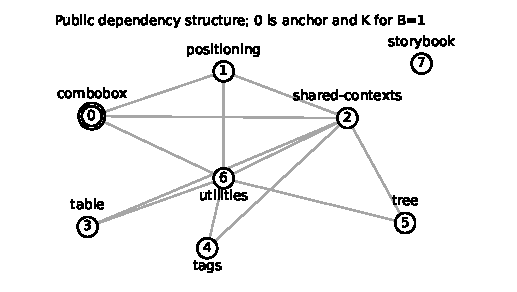
\includegraphics[width=\columnwidth]{images/ownership_case_v8.pdf}
\caption{Eight packages with publicly listed alternative owners~\cite{fluentuiowners}. Edges are in-portfolio runtime dependencies, symmetrized with unit proxy cost. The double circle is the synthetic change anchor and retained region for $B=1$. Routing labels and cost changes are illustrative.}\label{fig:ownership}
\end{figure}

We retain all eight anchors, increases 4/12 and budgets 1--4 (64 repairs), checking every binary assignment and both guarded CP routes. Values match throughout; 40 budgets strictly raise the optimum and 8 use the shared shortcut. This is an exploratory mechanism illustration, not a measured workload: an earlier cost-4 diagnostic had 64/64 shortcuts and is also retained. No runtime gain or operational event frequency is inferred. Source blobs, owner-rule lines, assumed quantities, both configurations and all outcomes are supplied.

\subsection{Public CAD Structure Audit}
The Bath logs~\cite{gopsill2019data,gopsill2019dsm} record three vehicle-design projects, not interchangeable teams. Retaining files with at least five distinct edit times yields 226/231/168 nodes. Each edit counts other files once until the next same-file edit or $h=1,12$ hours; averaged directional frequencies are thresholded at $1/4$ and rounded after scaling by eight. Isolates remain. Edge counts are 2726/8152, 535/693 and 199/481: co-edit proxies, not physical interfaces (Fig.~\ref{fig:public}). Synthetic preferences/costs, one/four anchors, $B=8,16$ and three seeds define 72 cases frozen before outcomes (full generator supplied). All CP pairs prove equal values, but 66 use the shared shortcut (14 without changes). Qualification and slack are unobserved. This shows structure compatibility, not operational acceleration or how frequently reduction helps.

\begin{figure*}[t]
\centering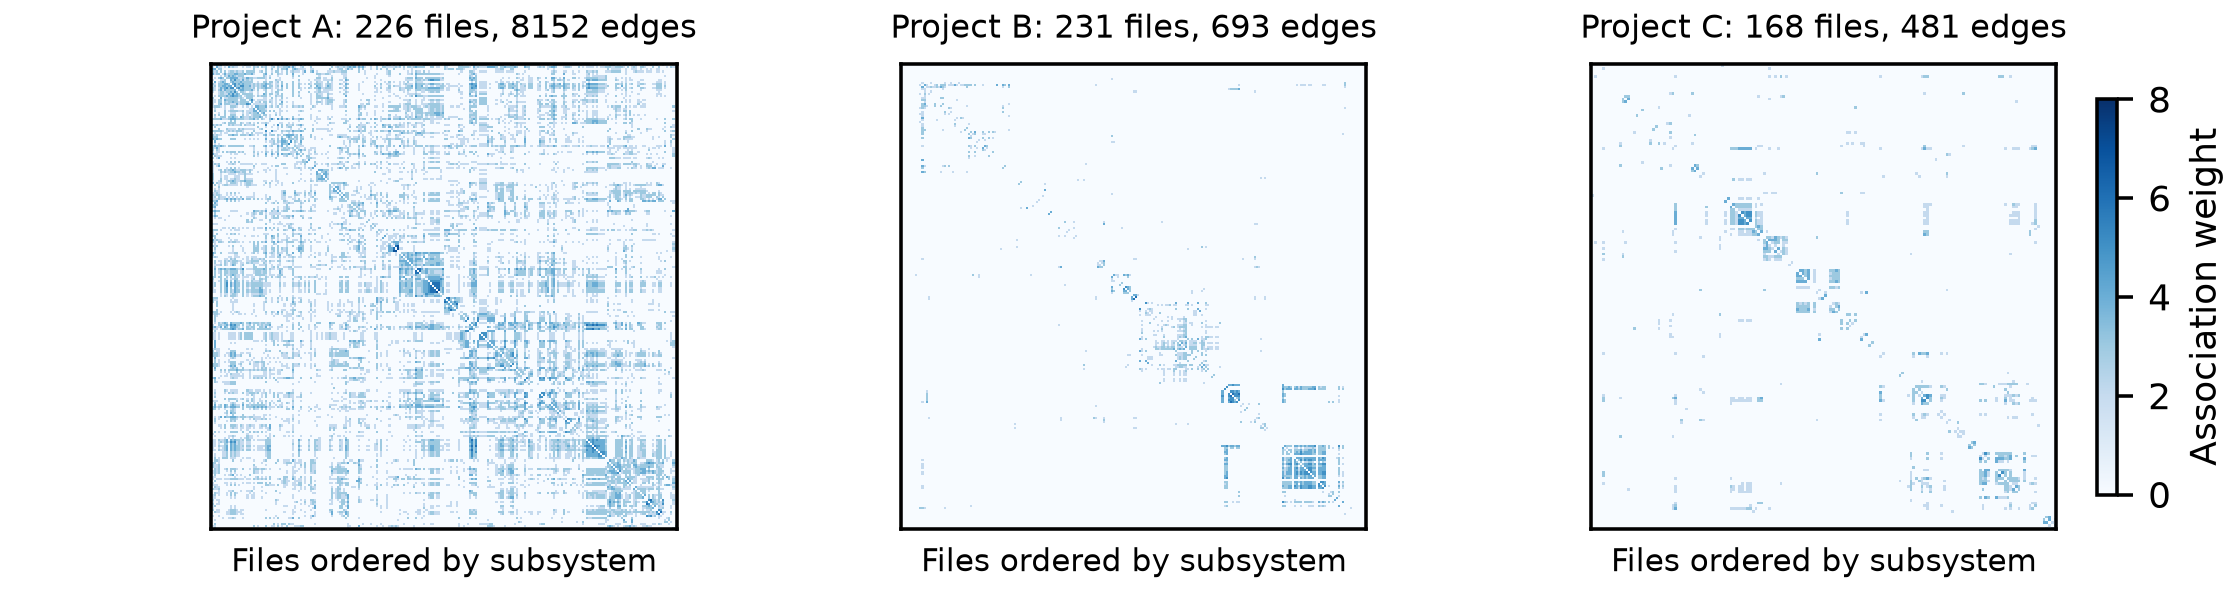
\includegraphics[width=\textwidth]{images/public_graphs_v5.png}
\caption{Twelve-hour CAD co-edit proxy matrices from public logs~\cite{gopsill2019data}, ordered by subsystem and file ID. Color shows quantized association weight, not measured handoff effort or physical interfaces. All qualifying files, including isolates, remain; binary ownership and costs are synthetic.}\label{fig:public}
\end{figure*}

\subsection{Lagrangian Route and Larger/Harder Inputs}
LRRepair is our classical comparator, not a named optimizer reproduction. Exact rational cuts of $E_1+\lambda R$ give lower bounds $q(\lambda)-\lambda B$. Doubling brackets a feasible cut, followed by at most 24 bisections. It retains the best feasible cut, restores the closest infeasible cut by minimum energy increase per freed effort, and uses feasible single-flip descent from that result, the old plan and feasible cut. Dual search gets at most 65\% of the target, recovery the remainder; the old plan is a fallback. Integer ceiling preserves the bound. Finite multiplier search need not optimize the dual; recovery has no approximation guarantee.

We compare all three routes freshly on every previous 120 large and 20 core inputs, plus the 72 public cases (636 calls). The scale grid is $n=1024,2048$, three families, one/four anchors, $B=16,64$, coupling 12, perturbation scale 64, heterogeneous costs, and five seeds. It was frozen after 32 exploratory cases. Core instances contain a $q=64,128$ cycle plus random matching, unit internal edges, anchor-star edges of weight 3, and a dominated tail to reach $n$. Core unaries are $(0,-1)$, tail $(0,10)$; anchor changes from $(0,4q+1)$ to $(0,-4q)$, with unit handoffs and $B=1+q/2$. The old all-zero plan is uniquely optimal; a new optimum changes the anchor and $q/2$ core vertices. Only $q$ controls intrinsic search difficulty; tail growth tests exterior preprocessing.

Targets are three seconds for scale/public and five for cores, with rotating method order and one timing each. These descriptive comparisons reuse earlier inputs; they are not additional independent instances or pooled with triple-timing intervals. Table~\ref{tab:routes} retains every censored call and reports quality alongside time.

\begin{table*}[t]
\caption{Fresh three-route comparison. F/R/L = FullCP/BARRCP/LRRepair; times are all-case median seconds. Cert counts each method's closed bounds; gap is its maximum returned absolute bound gap, retaining all incomplete calls. $K$ is the CP-required median region percentage; -- means every case uses the shortcut. Faster feasible outcomes need not have equal quality.}\label{tab:routes}
\centering\footnotesize
\begin{tabular}{@{}lrrrrrr@{}}
\toprule Input & $n$ & CP/all & $K$\% & Cert F/R/L & Time F/R/L (s) & Max gap F/R/L\\\midrule
% BEGIN GENERATED ROUTE ROWS
Grid & 1024 & 20/20 & 70.5 & 20/20/11 & 0.189/0.115/0.081 & 0/0/7 \\
Grid & 2048 & 16/20 & 50.4 & 20/20/15 & 0.289/0.067/0.187 & 0/0/3 \\
Modular & 1024 & 15/20 & 13.7 & 20/20/6 & 0.075/0.012/0.059 & 0/0/26 \\
Modular & 2048 & 14/20 & 7.1 & 20/20/6 & 0.148/0.016/0.126 & 0/0/24 \\
Small-world & 1024 & 20/20 & 100.0 & 20/20/6 & 0.256/0.268/0.143 & 0/0/17 \\
Small-world & 2048 & 20/20 & 100.0 & 16/16/10 & 0.639/0.627/0.320 & 418/418/8 \\
Core 64 & 1024 & 5/5 & 9.4 & 5/5/0 & 0.440/0.215/0.082 & 0/0/21 \\
Core 64 & 2048 & 5/5 & 4.7 & 5/5/0 & 0.641/0.221/0.173 & 0/0/21 \\
Core 128 & 1024 & 5/5 & 18.8 & 2/4/0 & 5.002/3.548/0.120 & 15/17/43 \\
Core 128 & 2048 & 5/5 & 9.4 & 1/4/0 & 5.004/3.756/0.235 & 20/17/43 \\
CAD A, 1 h & 226 & 0/12 & -- & 12/12/12 & 0.0013/0.0013/0.0018 & 0/0/0 \\
CAD A, 12 h & 226 & 0/12 & -- & 12/12/12 & 0.0036/0.0037/0.0051 & 0/0/0 \\
CAD B, 1 h & 231 & 2/12 & 24.9 & 12/12/10 & 0.0004/0.0004/0.0005 & 0/0/15 \\
CAD B, 12 h & 231 & 3/12 & 66.2 & 12/12/11 & 0.0004/0.0004/0.0006 & 0/0/1 \\
CAD C, 1 h & 168 & 0/12 & -- & 12/12/12 & 0.0002/0.0002/0.0003 & 0/0/0 \\
CAD C, 12 h & 168 & 1/12 & 43.5 & 12/12/12 & 0.0003/0.0003/0.0005 & 0/0/0 \\
% END GENERATED ROUTE ROWS
\bottomrule\end{tabular}
\end{table*}

At 2,048 vertices, 14/20 modular cases require CP; their median paired FullCP/BARRCP speed is 7.30 (earlier 7.67), with all-case medians 0.148/0.016 s. On 64-cores at that size both CP routes certify 5/5, with median paired speed 3.24 (earlier 2.86). LRRepair's median is 0.173 s but maximum actual loss is 12 against proved optima, with no certificates. It loses up to 26 on the eight 128-core cases with a proved reference optimum. BARRCP certifies 4/5 per size in this single run (previously 1/5), motivating repeats; these separate stages establish neither stable success probability nor its cause.

LRRepair matches 71/72 public optima, certifies 69/72 and loses at most one. It matches every proved grid optimum, with some dual bounds open. On four censored 2,048-vertex small-world cases it improves both CP incumbents by up to 417; its maximum gap is 8 versus 418 for CP, and reduction remains ineffective. Cut recovery can favor fast feasible repair, BARR exact certification on suitable structures; neither dominates time, quality and bound closure.


\subsection{Repeatability of Difficult Core Queries}
All 20 saved cores are repeated ten times per CP route (400 calls), with the same five-second target, one worker and fixed solver seeds. The frozen protocol shuffles cases and alternates methods. Suspend-affected diagnostics are archived separately. Continuous monotonic time and clock/pause checks (0.1 s threshold) pass for all 400 calls, completed in two segments after a tool interruption without rerunning saved calls. No concurrent benchmark or document build was launched.

\begin{table*}[t]
\caption{Repeated core queries: five fixed instances per row, ten repeats per method. F/R = FullCP/BARRCP. Closed counts are out of 50 calls; ranges give per-instance counts out of ten. Time is median [Q1,Q3] of all query totals, including incomplete calls, not uncensored time-to-optimum. Rel.~IQR is the median across instances of each instance's (Q3--Q1)/median time (\%). These are descriptive repeats, not 50 independent instances.}\label{tab:repeat}
\centering\footnotesize\setlength{\tabcolsep}{2pt}
\begin{tabular}{@{}rrrrlrr@{}}
\toprule $q$ & $n$ & Closed F/R & Per-case F/R & Query time F / R (s) & Rel.~IQR F/R & Max gap F/R\\\midrule
% BEGIN GENERATED REPEAT ROWS
64 & 1024 & 50/50 & 10--10/10--10 & 0.453 [0.311,0.604] / 0.216 [0.211,0.238] & 2.4/1.9 & 0/0 \\
64 & 2048 & 50/50 & 10--10/10--10 & 0.615 [0.545,0.783] / 0.218 [0.214,0.242] & 1.5/4.0 & 0/0 \\
128 & 1024 & 18/40 & 0--9/0--10 & 5.002 [4.393,5.002] / 3.517 [3.018,4.073] & 0.0/2.6 & 17/17 \\
128 & 2048 & 15/39 & 0--9/0--10 & 5.004 [4.945,5.004] / 3.548 [3.006,3.922] & 0.0/1.3 & 20/17 \\
% END GENERATED REPEAT ROWS
\bottomrule\end{tabular}
\end{table*}

Table~\ref{tab:repeat} retains all incomplete queries. Small dispersion at the cap reflects censoring, not reliable time-to-optimum. Uncontrolled background load/power and fixed-seed single-laptop repeats preclude cross-session reliability claims. Closure uses each call's own interval. We give no unresolved-core speed ratio or independent-trial interval; all per-case outcomes and timing components are supplied.

\section{Discussion and Limitations}
The contribution is a value-preserving/additively certified preprocessing rule, not a claim that every optimum is local or that constrained search becomes polynomial. Dense connectivity can retain the full graph. Repeated events require recertification: a previous budgeted optimum need not be the next old unconstrained optimum.

The ownership case documents alternative responsibility roles; its costs and capacities remain hypothetical. The capacity check converts a slack assumption into a test only when real loads and reservations are supplied. CAD co-edits alone establish neither eligibility nor human efficiency. Practical value is conditional: a budget must exclude the returned cut, the retained region must shrink, and saved search must exceed preprocessing. Active capacities, scheduling and multiple teams require a new feasibility argument. There is no industrial transfer trial or peak-memory benchmark. Single route timings and two-segment repeats on one laptop do not establish cross-machine stability. Tighter old certificates and feasible sets closed under union reversion remain open directions.

\section{Conclusion}
Union reversion, weighted paths and boundary absorption yield a certified region reduction for localized binary responsibility repair. Matched experiments support conditional benefits on modular/grid structures. Public ownership records ground a proposed use, while a capacity check makes its static-slack requirement testable. Operational gains and active-capacity extensions remain unestablished.

\begin{thebibliography}{15}
\bibitem{githubowners} GitHub, ``About code owners,'' GitHub Docs. [Online]. Available: \url{https://docs.github.com/articles/about-code-owners}. Accessed: Oct. 30, 2026.
\bibitem{fluentuiowners} Microsoft, ``Fluent UI: CODEOWNERS and package manifests,'' commit \texttt{941ed35}, Oct. 30, 2026. [Online]. Available: \url{https://github.com/microsoft/fluentui/tree/941ed35fd8973ccd899fafafc1ae7c8f58e5c1f2}.
\bibitem{kolmogorov2004graphcuts} V. Kolmogorov and R. Zabih, ``What energy functions can be minimized via graph cuts?'' \emph{IEEE Trans. Pattern Anal. Mach. Intell.}, vol. 26, no. 2, pp. 147--159, 2004.
\bibitem{gopsill2019dsm} J. A. Gopsill, C. Snider, and B. J. Hicks, ``The emergent structures in digital engineering work: what can we learn from dynamic DSMs of near-identical systems design projects?'' \emph{Design Science}, vol. 5, 2019, doi: 10.1017/dsj.2019.20.
\bibitem{gopsill2019data} J. Gopsill, C. Snider, and B. Hicks, ``Dataset for the emergent structures within digital engineering work: what can we learn from dynamic DSMs of near-identical systems design projects?'' University of Bath Research Data Archive, 2019, doi: 10.15125/BATH-00621.
\bibitem{zhang2025sharing} L. Zhang and L. Liang, ``Solving inter-group personnel sharing task allocation problem via group multirole assignment,'' in \emph{Proc. CSCWD}, 2025, pp. 1118--1123, doi: 10.1109/CSCWD64889.2025.11033310.
\bibitem{liu2025time} H. Liu and L. Liang, ``Fine-grained group role assignment based on time-oriented cooperation and conflict,'' in \emph{Proc. CSCWD}, 2025, pp. 1160--1165, doi: 10.1109/CSCWD64889.2025.11033475.
\bibitem{hannan2026divisible} S. Hannan and W. Chen, ``Task allocation for scalable edge computing with divisible group role assignment,'' in \emph{Proc. CSCWD}, 2026, pp. 2532--2537, doi: 10.1109/CSCWD68734.2026.11582688.
\bibitem{fischetti2003local} M. Fischetti and A. Lodi, ``Local branching,'' \emph{Mathematical Programming}, vol. 98, pp. 23--47, 2003, doi: 10.1007/s10107-003-0395-5.
\bibitem{gorelick2014submodularization} L. Gorelick, Y. Boykov, O. Veksler, I. Ben Ayed, and A. Delong, ``Submodularization for binary pairwise energies,'' in \emph{Proc. IEEE CVPR}, 2014, pp. 1154--1161.
\bibitem{kakimura2022reassignment} N. Kakimura, N. Kamiyama, Y. Kobayashi, and Y. Okamoto, ``Submodular reassignment problem for reallocating agents to tasks with synergy effects,'' \emph{Discrete Optimization}, vol. 44, Art. no. 100631, 2022.
\bibitem{tu2025optirefine} S. Tu, A. Stankovic, S. Neumann, and A. Gionis, ``OptiRefine: Densest subgraphs and maximum cuts with $k$ refinements,'' \emph{Data Mining and Knowledge Discovery}, vol. 39, Art. no. 82, 2025.
\bibitem{zhang2018screening} W. Zhang, B. Hong, L. Ma, W. Liu, and T. Zhang, ``Safe element screening for submodular function minimization,'' in \emph{Proc. ICML}, PMLR vol. 80, 2018, pp. 5786--5795.
\bibitem{kohli2007dynamic} P. Kohli and P. H. S. Torr, ``Dynamic graph cuts for efficient inference in Markov random fields,'' \emph{IEEE Trans. Pattern Anal. Mach. Intell.}, vol. 29, no. 12, pp. 2079--2088, 2007.
\bibitem{deberg2026stable} M. de Berg, A. L\'opez Mart\'inez, and F. Spieksma, ``Stable and dynamic minimum cuts,'' \emph{J. Graph Algorithms Appl.}, vol. 30, no. 1, pp. 89--107, 2026.
\end{thebibliography}
\end{document}
